\begin{abstract}
    Mutations can be beneficial by bringing an innovation to their bearer, allowing them to adapt to changes in environments or in selective pressure.
    However, mutations can also be beneficial because they are repairing previous deleterious changes, simply restoring existing functions.
    In this study, we first estimated selective effects of mutations inside mammalian protein coding sequences, under a model assuming no adaptation at the phylogenetic scale.
    We then estimated the proportion of beneficial mutations that are not adaptive innovations among all beneficial mutations at the population scale.
    Our work confirms that deleterious substitutions have accumulated in mammals and are currently being eliminated.
    In modern humans, it results in around 25\% of beneficial mutations that are not adaptive innovations, but instead are repairing previous deleterious changes.
\end{abstract}

\keywords{Adaptation \and Back-mutation \and Phylogenetics \and Population-genetics \and Codon models }

Adaptation is considered one of the main processes shaping the diversity of forms and functions across the tree of life\cite{darwin_origin_1859}.
It enables species to access new ecological niches and also respond to changes in their environment\cite{gavrilets_adaptive_2009}.
In evolution, adaptation is tightly linked to the notion of change at the level of the environment and to species responding to this change\cite{merrell_adaptive_1994}.
The process of adaptation leaves marks of accelerated evolution in genomes since mutations that are beneficial under new conditions fix faster than neutral mutations (fig.~\ref{fig:fitness-landscape}A).
The signature of an accelerated rate of substitutions can thus be interpreted as a sign of adaptation\cite{mcdonald_adaptative_1991, smith_adaptive_2002, welch_estimating_2006}.
The current availability of large-scale genomic data and the development of theoretical models have allowed to detect and quantify acceleration of substitution rates across genes and lineages, and these analyses have become common practice in evolutionary biology\cite{yang_statistical_2000, eyre-walker_genomic_2006, moutinho_variation_2019}.
Although these approaches have led to a better understanding of the processes determining the rates of molecular evolution, they have had the collateral effect of associating beneficial mutations with adaptive evolution.
We argue that we should dissociate beneficial mutations from adaptive mutations since adaptive evolution is not the only process that can lead to beneficial mutations\cite{charlesworth_other_2007, mustonen_fitness_2009}, and in turn, limit the use of adaptive mutations to those that are associated with adaptation to environmental change as such.
We here suggest that many beneficial mutations are not adaptive, but are rather restoring ancestral states of higher fitness.
We used large-scale genomic data to integrate analyses at both the phylogenetic and population scales to differentiate between truly adaptive mutations from mutations restoring the ancestral fitness.
Our results show that between 10 and 25\% of beneficial mutations in mammalian populations are not driven by adaptive innovations, but rather compensate the effect of ancestral deleterious mutations.

In a constant environment, a deleterious mutation can reach fixation in the population by genetic drift\cite{Ohta1992}.
Subsequently, a new mutation that is restoring the ancestral fitness will thus be beneficial (fig.~\ref{fig:fitness-landscape}B), even though no change in the environment has occurred\cite{hartl_compensatory_1996, sella_application_2005, mustonen_fitness_2009, cvijovic_fate_2015}.
The restoration of the ancestral fitness can happen either at a different locus than the initial mutation, in which case it is referred to as a compensatory mutation\cite{hartl_compensatory_1996, mustonen_fitness_2009}, or at the same locus than the initial mutation, referred to as a beneficial back-mutation\cite{piganeau_estimating_2003, charlesworth_other_2007}.
While compensatory mutations induce genetic changes at the sequence level, and thus genetic diversification, beneficial back-mutations reduce the genetic diversity and do not contribute to genetic innovation.
In this study, we focus on beneficial back-mutations, which merely cancel the effect of the previous deleterious changes.
Altogether, we argue that not all beneficial mutations contribute to genetic innovation, and thus that the extent of adaptive evolution can only be correctly estimated if we can account for the number of beneficial back-mutations\cite{keightley_what_2010, rice_evolutionarily_2015}.

Given a beneficial mutation, whether it is a new innovation responding to a change in environment or a beneficial back-mutation has the same consequences on its bearer\cite{charlesworth_other_2007}.
Similarly, at the level of the population, both types of mutation will result in a positive transmission bias of the beneficial allele.
However, at the macro-evolutionary scale the consequences of these two types of mutations are fundamentally different.
While adaptive evolution promotes phenotype diversification (fig.~\ref{fig:fitness-landscape}C), beneficial back-mutations promote phenotype stability and may help preserve well established biological systems (fig.~\ref{fig:fitness-landscape}D).
Additionally, the direction of adaptive evolution is unpredictable because it is caused by an unpredictable change in the environment and, hence, in the underlying fitness landscape\cite{bazykin_changing_2015}.
On the other hand, beneficial back-mutations are predictable if the underlying stable fitness landscape is known because we will expect to see changes from non-optimal amino acids to optimal ones.
If we wish to quantify the amount of beneficial back-mutations that have happened along a phylogeny we need to identify the selection coefficients of mutations and to achieve this we require the fitness landscape to be stable and be known.

The placental mammals represent an excellent study system to perform this analysis.
Having originated $\sim$100 Mya\cite{kumar_timetree_2017}, they diversified quickly.
Additionally, we have polymorphism data available for many species\cite{howe_ensembl_2021} and high quality protein-coding DNA alignments across the genome\cite{ranwez_orthomam_2007, scornavacca_orthomam_2019}.
By restricting our analysis to protein-coding orthologous genes to all the phylogeny, and further excluding any genes for which there have been claims of pervasive directional selection, we can not only assume a constant fitness landscape for each of them throughout placental mammal evolution, but actually reconstruct the fitness landscape from variable positions within the sequence along the phylogeny.
For each gene, we used a codon model of mutation-selection\cite{halpern_evolutionary_1998, mccandlish_modeling_2014} to obtain relative fitnesses for all amino-acids for each site of the sequence by fitting the model to the multi-species sequence alignment (fig~\ref{fig:method}A) and assuming that the underlying fitness landscape is stable along the phylogenetic tree.
%Mutation-selection codon models provide a nearly neutral framework of evolution taking into account non-adaptive processes impacting codon frequency\cite{halpern_evolutionary_1998, rodrigue_mechanistic_2010, tamuri_estimating_2012, latrille_improved_2022}.
From the fitness landscape, we can calculate the scaled selection coefficient $\Sphy$ for any possible amino-acid change at each position.
Under this model, a mutation with a positive $\Sphy$ would be driving the current site toward a known fitter amino-acid and would thus be considered as a beneficial back-mutation (fig~\ref{fig:method}B), given the assumed stability of the fitness landscape.

Having identified which potential amino-acid changes could represent beneficial back-mutations at the phylogenetic scale, we retrieved polymorphism data from 28 populations belonging to 6 genera (\textit{Equus}, \textit{Bos}, \textit{Capra}, \textit{Ovis}, \textit{Chlorocebus} and \textit{Homo}) to assess the presence of beneficial back-mutations at the population scale.
We focused on currently segregating mutations within populations and also on substitutions in the terminal lineages, and checked if any of these observed changes where predicted beneficial back-mutations.
Essentially, by integrating large scale genomic datasets at both phylogenetic and population scales we have been able to estimate the amount of beneficial back-mutations across the entire exome for 6 different mammalian genera (fig~\ref{fig:method}A-F).

Our analyses allow us to test long-standing questions in molecular evolution:
How common are beneficial back-mutations?
Can we identify beneficial back-mutations that have reached fixation recently, and ones that are currently segregating in populations?
Are hypothetical beneficial back-mutations effectively beneficial for the individuals carrying them?
Furthermore, what is the probability for any beneficial mutation observed in current populations to be a back-mutation?
In other words, can we quantify the amount of beneficial mutations that are restoring damaged genomes instead of creating adaptive innovations.
By addressing these questions we provide
novel insight on how selection is affecting protein-coding DNA sequences.

\begin{figure*}[!ht]
    \centering
    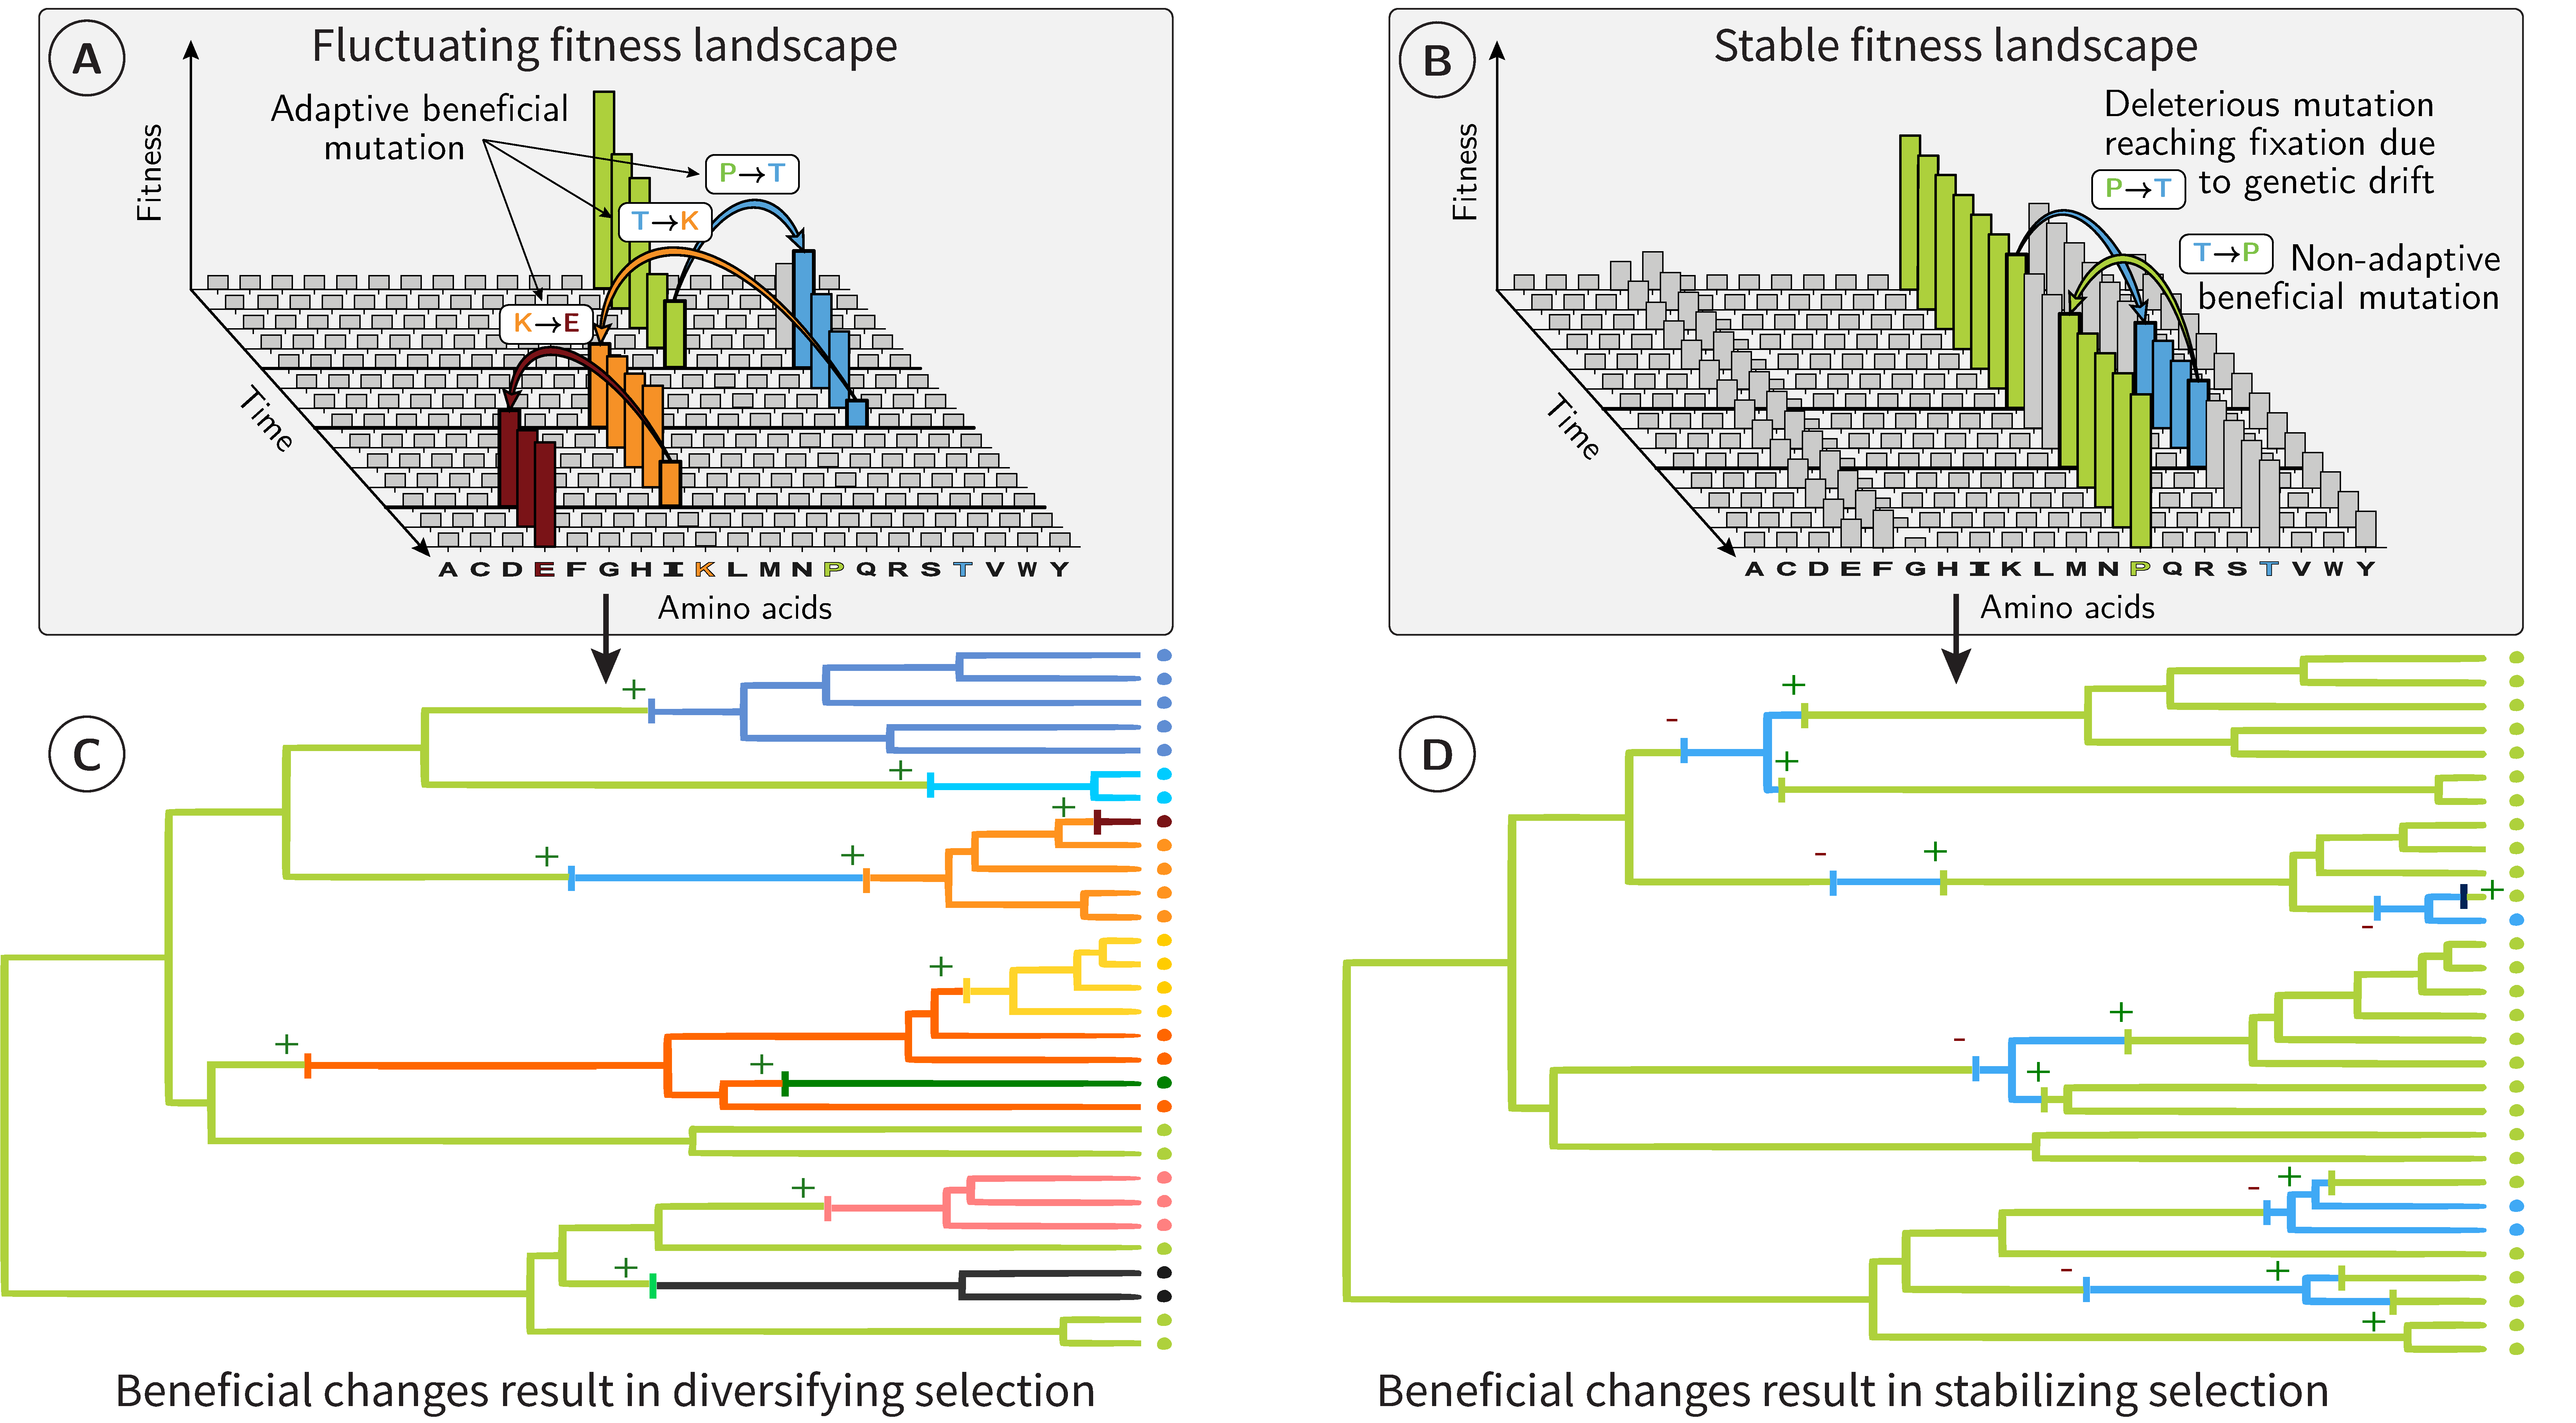
\includegraphics[width=\textwidth, page=1] {artworks/figure.fitness-landscape}
    \caption{
        Panel A and B: at a given site of a protein-coding DNA sequence, the different amino-acids (x-axis) have different fitnesses (y-axis).
        Under a fluctuating fitness landscape (panel A), these fitnesses are changing with time.
        The protein sequence is always lagging behind the moving target defined by the amino-acid fitnesses, and since substitutions are accepted preferentially if they are in the direction of this target, substitutions are on average adaptive.
        At the phylogenetic scale (panel C), this phenomena promotes phenotype diversification across species.
        Under a stable fitness landscape (panel B), all the mutations reaching fixation are either slightly deleterious and reaching fixation due to drift, or are beneficial back-mutations restoring a more optimal amino-acid.
        At the phylogenetic scale (panel D), this phenomena promotes promotes phenotype stability and preserves well established biological systems.
        At the genome level, slightly deleterious mutations that have reached fixation are supposedly scattered at different loci, such that beneficial back-mutations should also be spread across the genome.
        We thus expect that the genome-wide signature of beneficial back-mutations can be detected and quantified, even though each mutation has individually a small beneficial effect on their bearer.
    }
    \label{fig:fitness-landscape}
\end{figure*}